\documentclass[a4paper,11pt]{article}
\usepackage{graphicx}
\graphicspath{ {../graphs/} }

\begin{document}
\title{Lab2 Report}
\author{Kailean O'Keefe}
\date{\today}
\maketitle

\section*{Introduction}
This lab focused on simulating the way that TCP transfers files as bytes across a network. It went in depth into how TCP sends data, the various buffers used when sending and receiving data, as well as what TCP does to handle the situation when a packet is lost. 

\section*{Basic Tests}
This first section had us setup a very basic version of TCP. This involved creating buffers to send and receive data as well as creating timers to track timeouts for packets sent across the connection.

\begin{table}[h!]
  \begin{center}
    \caption{Loss Percentages}
    \label{tab:table1}
    \begin{tabular}{l|c|c|c|r} % <-- Alignments: 1st column left, 2nd middle and 3rd right, with vertical lines in between
      \textbf{Method} & \textbf{0\%} & \textbf{10\%} & \textbf{20\%} & \textbf{30\%}\\
      \hline
      Basic & 7.367232 & 108.156896  & 226.1771328 & 418.6470464\\
      Fast & 7.367232 & 44.619776  & 75.7146496 & 119.6228096\\
    \end{tabular}
  \end{center}
\end{table}

As shown in the table above in the basic row, as the loss percentage increases, the overall time required to transmit the file also increases dramatically. It is also worth mentioning that there are times when the receiver sends one ACK for multiple MSS's. This phenomenon is caused by the receiver receiving packets out of order. When the retransmission timer fires, the sender retransmits the missing packet that caused the disorder, and the receiver puts the missing MSS in order. The Receiver then sends an ACK for the next MSS it's looking for which causes multiple MSS's to be received under the same ACK.  

\section*{Fast Retransmission}
Fast retransmit was implemented in mostly the same way as the basic version, however fast retransmit also had some extra logic designed to handle the case of a "triple double ACK". A "triple double ACK" occurs when the receiver asks for the same packet 4 times in a row. This when this occurs, the fast retransmit registers that as a dropped packet and immediately calls retransmit. This small optimization allows for the program to predict some of the packet loss and gain back some time that would otherwise be lost. It is also worth mentioning that this change is particularly effective when the loss rate is low -- however as shown in the table above -- the time that this optimization can save is significant across the board.

\section*{Experiments}
The last section of this lab involved playing with the alloted window size for the transfer. The experiments involved transferring the\\ internet-architecture.pdf file using the following window sizes 1000, 2000, 5000, 10000, 15000, and 20000. For each size, we graphed the queueing delay, and the throughput against the window size. Both of those graphs are provided below. 

\begin{center}
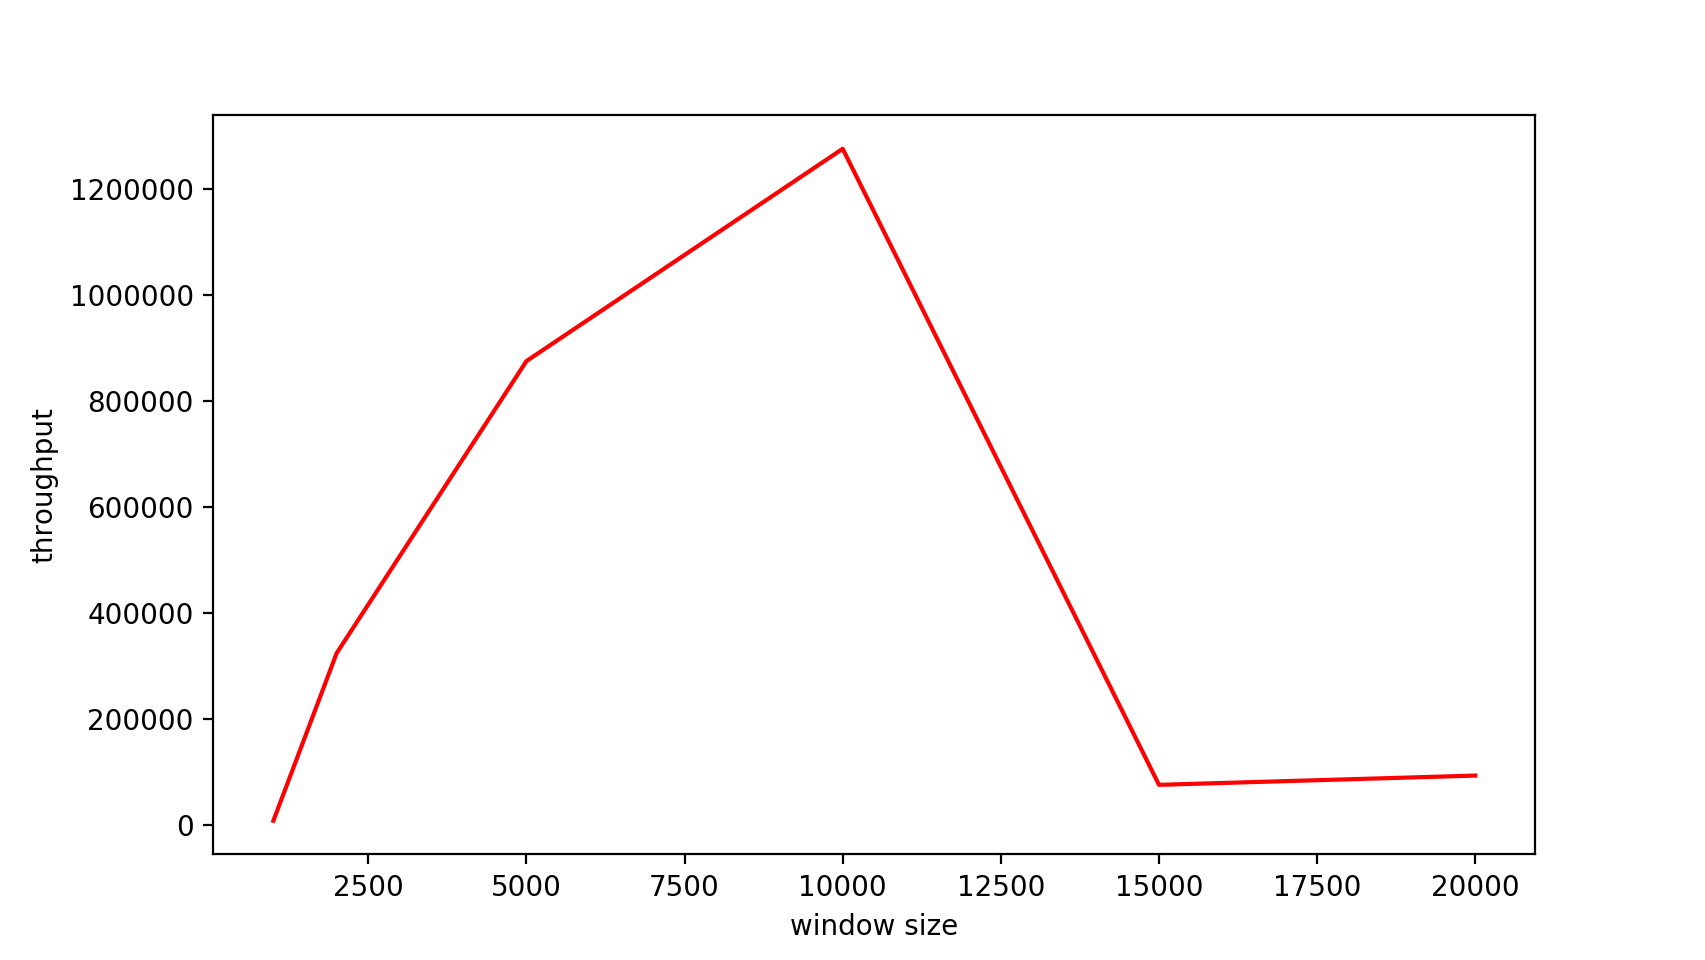
\includegraphics[width=\linewidth]{Throughput}
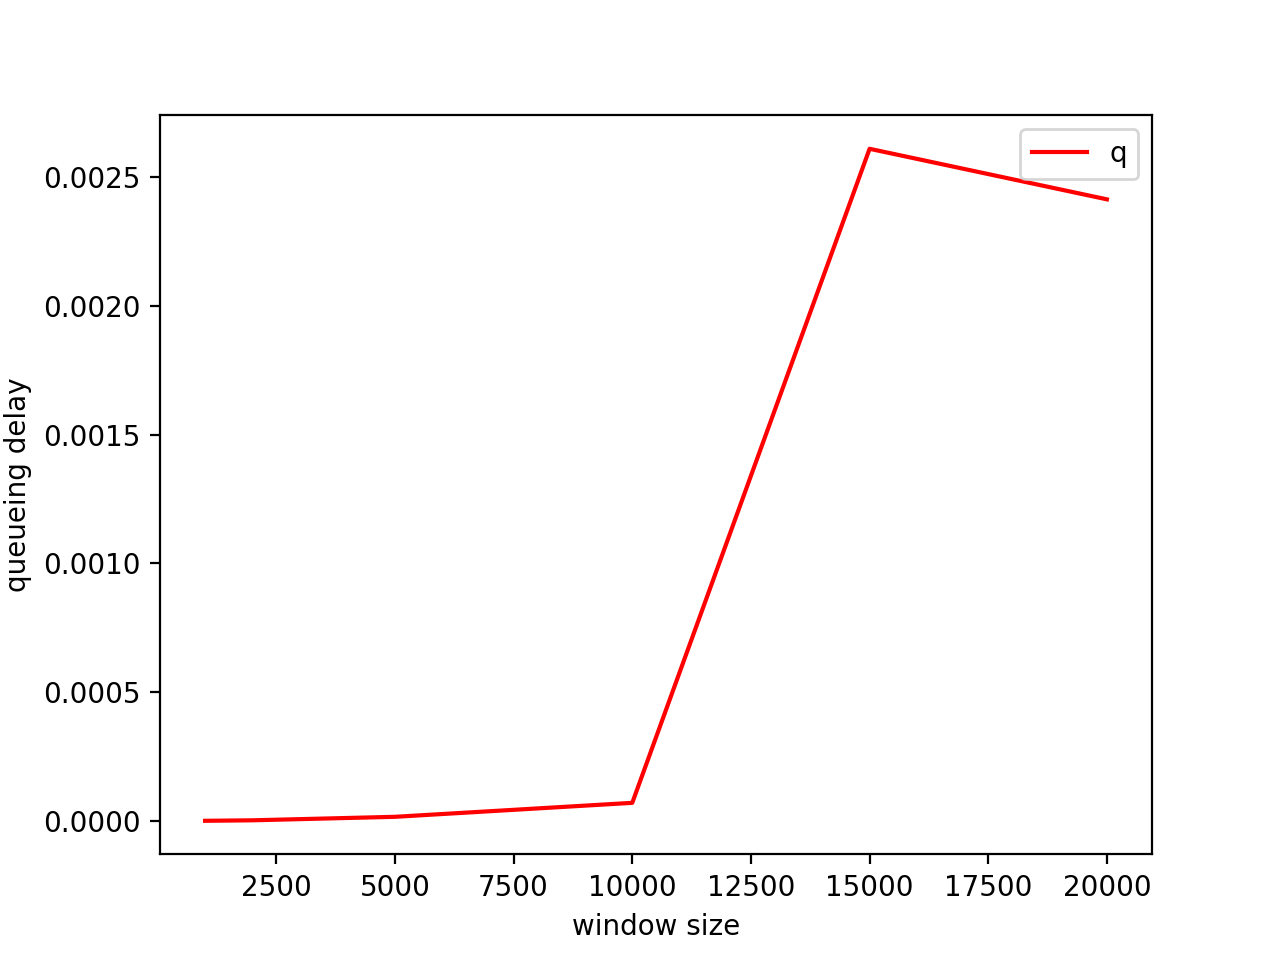
\includegraphics[width=\linewidth]{qd}
\end{center}

As seen in the graphs increasing the window size can help increase throughput to a point, however eventually the queuing delay incurred by having such a large window will start to counteract the benefits of having a large window. 

\section*{Conclusion}
It is important when designing TCP to be mindful of the various optimizations that can be added in to help decrease the amount of time necessary to transfer packets. According to the findings in this lab, the optimal solution would be to implement TCP using the fast transmit method, and to have your window size somewhere around 10000 bits. Implementing TCP in this way will allow you to not only maximize your throughput, but will also help your protocol quickly recover from packet loss.
\end{document}
